\documentclass[12pt]{article}

\usepackage{sbc-template}

\usepackage{graphicx,url}

%\usepackage[brazil]{babel}   
\usepackage[latin1]{inputenc}  

     
\sloppy

\title{Comparison of Methods of Noise Classification}

\author{Antonio Nascimento\inst{1}, Felipe de S. Farias\inst{1}, Marilia Alves \inst{2}}


\address{Programa de Pos-Graduacao em Engenharia de Defesa \\ Instituto Militar de Engenharia (IME)\\
\nextinstitute
  Programa de Pos-Graduacao em Engenharia Eletrica \\ Instituto Militar de Engenharia (IME)
\nextinstitute
  \email{\{antonio.nascimento,felipe.farias,marilia.alves\}@ime.eb.br}
}

\begin{document} 

\maketitle

\begin{abstract}

%This is the paper model for SBC conferences. I made some instructions so we can use it to write our own paper. It contains a suggestion of placement of the sections. 

Ok here we make the abstract. Needless to say it comes last. Should have max 10 lines.

\end{abstract}
     


\section{Introduction} \label{sec:intro}


%I took some liberties in the sketch Nascimento gave us in the Telegram group, combining with this paper \cite{nakagawa2012speaker} to come up with this model you're seeing. Initially, this Section describes the problem we are attempting to solve. We have to describe the problem many audio signal processing tasks face when performed in noisy conditions. References are much appreciated.

%After that, we should write some kind of small version of the next sections. Do it ONLY after writing all the other parts. Each paragraph in the other sections become some lines here.

Many Acoustic Signal Processing (ASP) tasks are performed in noisy conditions. The presence of noise, additive or otherwise, decreases the performance of those tasks, be it speaker recognition \cite{ming2007robust}, emotion recognition \cite{schuller2010cross}, source localization \cite{benesty2000adaptive} or speech recognition \cite{friesen2001speech}. Thus, it is imperative to study noise so we can better assess how it affects ASP tasks and how we can deal with it. Automatic classification of types of noise is an important part of this study, since the knowledge of the kind of noise present in a given situation is useful knowledge to better treat it \cite{may2012noise}.

There is extensive previous work in the field of audio classification. There is great variety in the methods used to perform this task, such as statistical methods \cite{dal1988acoustic,peltonen2002computational}, methods using stochastical knowledge such as \textit{Hidden Markov Models} (HMM) \cite{ma2003context}, using neural networks \cite{beritelli2005adaptive} and support vector machines \cite{cumani2012analysis}. There is variety also in the applications sought, such as speaker recognition \cite{kinnunen2010overview,murty2006combining,farrell1994speaker}, acoustic scene recognition \cite{piczak2015environmental,barchiesi2015acoustic} or animal species recognition \cite{somervuo2006parametric,lee2008automatic}. The noise classification is different only in application, but can be performed using any method used for audio classification \cite{beritelli2007adaptive,ma2006acoustic}.

This work proposes to evaluate the performance of four common methods used in audio classification in the specific task of classify noise. To this end, we implement those methods in the same set of audio files containing different types of noise. These files are taken from the NOISEX database \cite{varga1993assessment}, a database comprised of audios of 15 types of noise. The evaluation follows these steps: The extraction of the the mel-cepstral coefficients of each audio file, construction of the models according to each method, classification and evaluation of the results. The methods compared are the Neural Network, Gaussian Mixture Model, Support Vector Machines and K-means.

The remainder of this paper is organized as follows. Section \ref{class} introduces the task of noise classification, as long as the methods used in this paper. Section \ref{exp} describes the experiments performed and the results obtained and, finally, in Section \ref{conc} we present our conclusions about the results found, as long as the future works.

\section{Noise Classification} \label{class}

In this section we should describe the audio classification task and how it applies to our specific problem, the noise classification.

Additionally, we have to describe each method we use, in subsections.

\subsection{Mel-Cepstral Coefficient Extraction} \label{class:melcepst}

Here we talk about mel-cepstral coefficients and how to use them to identify each class of noise.

\subsection{Neural Network} \label{class:nn}

One or two paragraphs should do. Don't forget the proper references (like this one \cite{lei2014novel}).

\subsection{K-means} \label{class:kmeans}

This is a method used in summarization. Didn't find references.

\subsection{Gaussian Mixture Models} \label{class:gmm}

This section describes the use of Gaussian mixture models (GMM) in the task of noise representation and classification. Here is a good journal article for further reference \cite{reynolds1995robust}.


\subsection{Support Vector Machines} \label{class:svm}

Here we have a paper in audio classification using SVM \cite{cumani2012analysis}.



\section{Experiments} \label{exp}

Here we will describe the experiments. It should contain an introductory paragraph containing the purpose of the experiments.

\subsection{Experimental Setup} \label{exp:setup}

This paragraph should have all the requirements to perform the experiment, including hardware, software and general conditions. Sometimes people put the database here, but i think it will provide greater value if we put it in it's own subsection.

\subsection{Database Description} \label{exp:data}

Here we describe the NOISEX database. Since it's an important part of this work, we should take our time to properly describe it.

\subsection{Evaluation Metrics} \label{exp:metric}

ISSO EH UMA SUGESTAO

Here we can describe how we evaluate the performance of each experiment.

\subsection{Results} \label{exp:res}

You may be wondering why have only the 'results' and not the 'experiments' subsection. This is because we already told the reader everything he has to know in the previous sections. Section \ref{class} describes the different methods and Sections \ref{exp:setup} and \ref{exp:data} describe the details of the experiments.


\begin{table}[ht]
\centering
\caption{Accuracy per class for the methods compared.}
\label{tab:acc}
\begin{tabular}{l|llll}
\hline
Class & K-means & GMM & Neural Network & SVM \\
\hline
Babble & 86,01\% & 98,90\% & & \\
Bucanneer 1 & 97,11\% & 99,31\% & & \\
Bucanneer 2 & 98,86\% & 99,69\% & & \\
Destroyer Engine & 99,64\% & 99,67\% & & \\
Destroyer Ops & 91,79\% & 97,66\% & &\\
F16 & 96,67\% & 99,10\% & &\\
Factory 1 & 59,06\% & 91,11\% & &\\
Factory 2 & 94,10\% & 95,26\% & &\\
HF Channel & 100,00\% & 99,99\% & &\\
Leopard & 98,69\% & 98,93\% & &\\
M109 & 93,89\% & 99,01\% & &\\
Machine Gun & 7,45\% & 99,77\% & &\\
Pink & 99,76\% & 98,38\% & &\\
Volvo & 90,78\% & 99,67\% & &\\
White & 99,95\% & 99,96\% & &\\
\hline
\textbf{OVERALL} & 87,78\% & 98,43\% & & \\
\hline
\end{tabular}
\end{table}

\begin{table}[h]
\centering
\caption{Model of confusion matrix PRA EU N TER Q FAZER ISSO DE NOVO}
\label{tab:confusion}
\resizebox{\textwidth}{!}{\begin{tabular}{l|lllllllllllllll}
\hline
& Babble & Buccaneer 1 & Buccaneer 2 & Destroyer Engine & Destroyer Ops & F16 & Factory 1 & Factory 2 & HF Channel & Leopard & M109 & Machine Gun & Pink & Volvo & White \\
\hline
Babble & & & & & & & & & & & & & & & \\
Buccaneer 1 & & & & & & & & & & & & & & & \\
Buccaneer 2  & & & & & & & & & & & & & & & \\
Destroyer Engine  & & & & & & & & & & & & & & & \\
Destroyer Ops & & & & & & & & & & & & & & & \\
F16 & & & & & & & & & & & & & & & \\
Factory 1 & & & & & & & & & & & & & & & \\
Factory 2 & & & & & & & & & & & & & & & \\
HF Channel & & & & & & & & & & & & & & & \\
Leopard & & & & & & & & & & & & & & & \\
M109 & & & & & & & & & & & & & & & \\
Machine Gun & & & & & & & & & & & & & & & \\
Pink & & & & & & & & & & & & & & & \\
Volvo & & & & & & & & & & & & & & & \\
White & & & & & & & & & & & & & & & \\
\hline
\end{tabular}}
\end{table}

\section{Conclusions} \label{conc}

Here we conclude the paper. I suck at this, so pls someone do it for me. The one thing I know is that we have to summarize our findings and link it to our problem stated in the introduction, telling the reader whether we were successful or not in the task we proposed in the beginning.

%exemplo de figura

%\begin{figure}[ht]
%\centering
%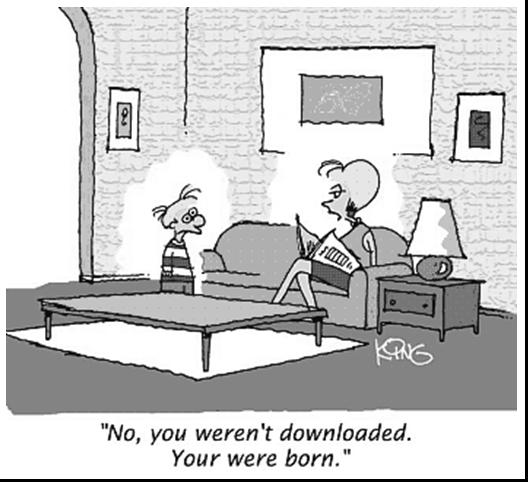
\includegraphics[width=.5\textwidth]{fig1.jpg}
%\caption{A typical figure}
%\label{fig:exampleFig1}
%\end{figure}

%\begin{figure}[ht]
%\centering
%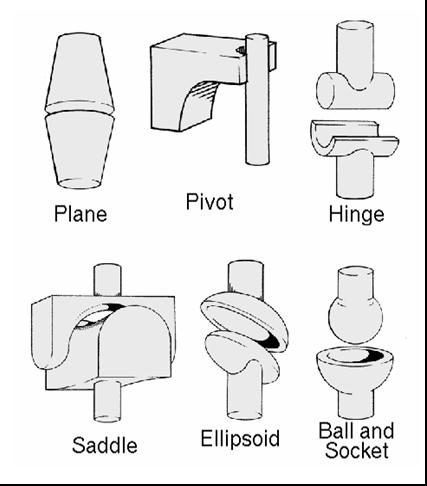
\includegraphics[width=.3\textwidth]{fig2.jpg}
%\caption{This figure is an example of a figure caption taking more than one
%  line and justified considering margins mentioned in %Section~\ref{sec:figs}.}
%\label{fig:exampleFig2}
%\end{figure}


% EXEMPLO DE TABELA

%\begin{table}[ht]
%\centering
%\caption{Variables to be considered on the evaluation of interaction  techniques}
%\label{tab:exTable1}
%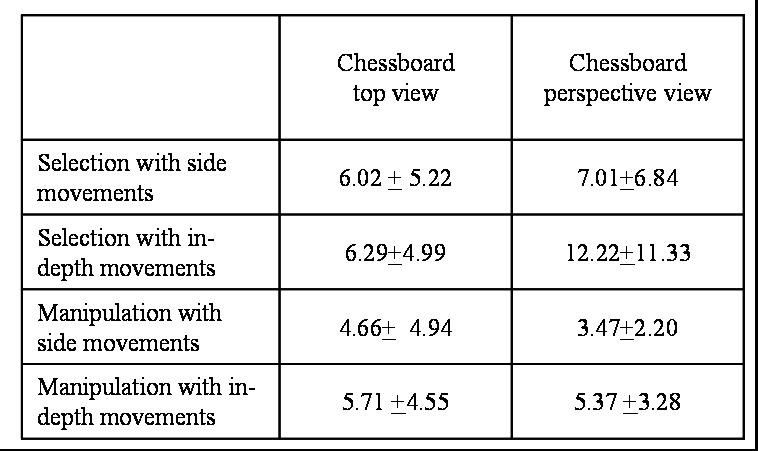
\includegraphics[width=.7\textwidth]{table.jpg}
%\end{table}



\bibliographystyle{sbc}
\bibliography{sbc-template}

\end{document}
